\documentclass[12pt,a4paper]{article}
\usepackage[utf8]{inputenc}
\usepackage{amsmath}
\usepackage{amsfonts}
\usepackage{amssymb}
\usepackage[english]{babel}
\usepackage{graphicx}
\usepackage{siunitx}
\usepackage{pdfpages}
\usepackage{listings}


\begin{document}
\begin{titlepage}

\centering \parindent=0pt
\newcommand{\HRule}{\rule{\textwidth}{1mm}}
\vspace*{\stretch{1}} \HRule\\[0.7cm]\Huge\bfseries
30010 - Programmeringsprojekt \\[0.7cm] % Kursusnummer og navn
Reflexball\\ % Titel
\HRule\\[2cm]  
\Large
Gruppe 3
\\
\large
Martin Boye Brunsgaard, s144012(1)	\\
Tore Gederaas Kanstad, s144021(2) \\
Peter Asbjørn Leer Bysted, s144045(3) \\
\begin{figure}[h]
\begin{center}
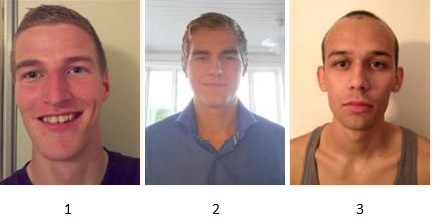
\includegraphics[scale=0.6]{img/faces.jpg}
\end{center}
\end{figure}

\vspace*{\stretch{1}} \normalsize

Alle medlemmer har været tilstede under øvelserne, og deltaget i udarbejdelse af journalerne. Ydermere har arbejdet været fordelt ligeligt over gruppemedlemerne, og løst i fællesskab. Rapporten er blevet udarbejdet og gennemlæst i kollektiv.
\vspace*{\stretch{1}}
\begin{flushleft}
Tecnical University of Denmark DTU\\ % Uddannelsesinstitusion
National Space Institute\\ 
30010 - Programming Project\\ % Kursusnummer og navn
25.06.2015 %Måned og år
\end{flushleft}
\end{titlepage}
\newpage
\renewcommand{\abstractname}{Abstract}
\begin{abstract}

This report covers the reflexbal game, which is a mandatory part of the B.Sc. EE course 30010 Programming Project.\\ The report documents the entire course of the exercises in which the digital logic behind a simple vending machine was designed using VHDL. The project was split into three sub-assignments: The first assignment was to drive a seven-segment display with hexadecimal numbers, the second was to display two different 2-digit decimal numbers simultaneously  and the last was to implement a CPU using a data path controlled by a FSM. The 3 assignements were combined into one circuit and implemented on a Basys2 Spartan FPGA board.
\end{abstract}
\newpage
\tableofcontents


\newpage
\section{Introduktion}
Målet med dette projekt er at designe og implementere et program. Programmet skal skrives i C og det skal implementeres på en Zilog Z8 encore microprocessor vha. ZDS II - Z8Encore! 4.9.3 værktøjer. Programmet skal dokumenteres vha. flowcharts, grafer og beskrivelser af de enkelte funktioner.

\begin{figure}[h]
\begin{center}
\includegraphics[scale=0.6]{img/reflexball.png}
\caption{Reflexball vist i PuTTY.}
\end{center}
\end{figure}

Programmet skal være et spil, Reflexball. Spilleren styrer en striker, som skal bruges til at reflektere en bold, således den kan bevæge sig rundt på banen. Hvis bolden rammer en af kanterne, skal bolden ligeledes også reflekteres. Hvis spilleren ikke rammer bolden ryger bolden ud af banen, og spilleren fratrækkes et liv. Såfremt spilleren ikke har flere liv tilbage, afsluttes spillet. Desuden indføres der nogle bokse i spillet, som spilleren skal ødelægge. Når spilleren har ødelagt alle disse bokse går spilleren videre til næste bane, eller vinder såfremt han er på sidste bane. Den grafiske flade bliver implementeret ved at skrive til en terminal. Ydermere får brugeren informationer fra LED'erne på boardet.


 
\section{Teori}

Vi vil i dette afsnit gennemgå den basale teori bag binære tal og slutteligt indføre læseren i de forskellige formater, deriblandt fixed-point format, og hvorfor det er interessant at bruge denne repræsentation  i vores projekt.
\subsection{Binære tal}
Et binært tal er et tal der kan udtrykkes i det binære talsystem/base-2, hvor grundtallet er 2. Da det er meget let at implementere i digital logik, er det et system der bruges internt i computere verden over. \\ 
Et binært tal består af bits, som svarer til et ciffer. Et bit kan have en af to tilstande: logisk højt eller logisk lavt. Dette medfører da hvis vi har \textit{n} bits har vi $2^n$ forskellige tilstande. Disse forskellige tilstande kan fortolkes på forskellige måder, og vi vil i de næste afsnit gennemgå nogle af de forskellige representationer.
\subsection{Unsigned repræsentation}
I det binære talsystem er grundtallet vanligvis 2(det kunne potentielt også være -2). Det betyder således at i en n-bit streng, vil  bittet yderst til højre være vægtet med  $2^0$, det næste med $2^1$ op til $2^n$ gående mod venstre. Tallet 5(base-10) kan da skrives som i ligning \ref{unsigned}. Ydermere tæller vi også fra højre mod venstre, og første bit står såldedes også på 0 plads. Dette bit kaldes oftest LSB(least significant bit), hvorimod det bit der står helt til venstre kaldes MSB(most significant bit).


\begin{equation}\label{unsigned}
5_{10} = 101_{2} = 1 \cdot 2^2+0 \cdot 2^1+1 \cdot 2^0
\end{equation}


Med de indførte definitioner har vi kun mulighed for at repræsentere positive heltal. Vi ønsker også at kunne skrive kommatal og negative tal.

\subsection{Fixed point kommatal}
Kommatal kan indføres på en simpel måde, ved blot at vægte i omvendt retning når man går mod højre, således at bittet til højre for kommaet har vægtningen $2^{-1}$, bittet 2 til højre for kommat vægtningen $2^{-2}$ osv. Hvis man har en n-bit streng med b tal til højre for kommaet, har man da muligheden for at skrive tal mellem 0 og $\frac{2^n-1}{2^b}$ \cite[s.~4]{Yates}

Tallet 13.625 kan f.eks skrives som

\begin{equation}
13.625_{10} = 1101.101_2 = 1 \cdot 2^3+1 \cdot 2^2+1 \cdot 2^0+1 \cdot 2^{-1}+1 \cdot 2^{-3}
\end{equation}

\subsection{Repræsentation af negative tal}
Hvis vi ønsker at repræsentere negative tal, gøres det oftest på 3 forskellige måder: 
Signed magnitude, 1's kompliment eller 2's kompliment. Vi vil her gennemgå signed magnitude og 2's komplement.
\subsubsection{Signed magnitude}
En af måderne at repræsentere fortegnet på bit-strengen, er ved at lade det mest signifikante bit(MSB: længst til venstre) bestemme fortegnet, hvor 0 indikerer et positivt tal og 1 indikerer et negativt tal.  F.eks. kan tallet -37 i signed magnitude repræsentation skrives således:
\begin{equation}
-37_{10} = 1100101_2 
\end{equation}
Signed magnitude repræsentation, har dog den ulempe, at man spilder et bit, f.eks. hvis man har en 4-bit streng gælder der at 1000 =  0000, så istedet for at have $2^4$ tilstande har man blot $2^4-1$. 
\subsubsection{2's komplement}
En anden måde at repræsentere negative tal, kan gøres vha. 2's komplement. 2's komplement findes ved at invertere et unsigned tal og derefter lægge 1 til. 2's komplement har to fordele: Der er kun et 0, og subtraktion kan gøres på samme måde som addition, så hvis vi ønsker at subtrahere 3 fra 5, skal vi blot finde 2's kompliment af 3 og lægge det til 5, som i \ref{2skomp}
\begin{equation}
\label{2skomp}
 5-3 = 5+(-3)
\end{equation}
Disse fordele gør 2's komplement et af de mest udbredte metoder til at repræsentere negative tal i digitale systemer.

\subsection{Fixed point vs floating}
SHIT HERE

%\newpage
\section{Design af Reflexball}
I udarbejdelsen af dette program havde vi nogle forskellige tekniske krav og mål, som vi ønskede at designe programmet efter.
\subsection{Tekniske mål}
Vi lavede en liste af krav til programmets design som vi i så høj grad som muligt ønskede at overholde. 
\begin{enumerate}
\item Vi ønsker en veldefineret struktur. Vi vil derfor undgå globale variable i så høj grad som muligt, derfor skal vi lave funktioner som tager pegere til strukturer eller variable som inputs, frem for at tilgå globale variable. Få undtagelser findes dog til dette, f.eks. i bibloteket der tilgår timeren.
\item Vi ville udvikle nogle moduler  der var uafhængige af hinanden, således at vores grafik i mindst mulig grad kommunikerede med vores modul indeholdende spillets back-end(Refball.c). Denne kommunikation skulle såfremt foregå igennem main-metoden, således man let kan få et overblik ved at se på main-metoden.
	
\end{enumerate}


\subsection{Krav til spillet}
\subsubsection{Overordnede krav til spillet}
\begin{enumerate}
\item Spillet er et arkanoid spil, bestående af 3 levels. Banerne skal være i stigende sværhedsgrad. Dette gøres ved at boksene gøres stærkere, således de skal rammes flere gange for at ødelægges, og også tilføje flere kasser.
\item Spilleren har 3 liv til at starte med, og får et liv for hver bane han vinder.
\item Hvis spilleren ikke har flere liv tilbage, afsluttes spillet og der vises game over på skærmen. Efter et par sekunder går spillet automatisk tilbage  til menuen.
\item Når banen begynder, eller hvis spilleren mister et liv, placeres bolden over strikeren, og spilleren kan frit bevæge strikeren, hvor bolden følger efter. Hvis spilleren trykker på den givne knap, affyres bolden i en opadgående lodret linje. 
\item Spillerens liv og tiden skal skrives på LED-skærmen når spillet er igang
\item Spilleren samler power hver gang han rammer en kasse. Hvis brugeren trykker på venstre og højre-tasten på en gang bruger han sit power og akitverer hiii power. Når hiii power er aktiveret ødelægges kasser når de rammes, uafhængigt af deres liv, og bolden reflekteres ikke, men fortsætter gennem kassen.
\item Når spilleren bruger hiii power, vinder en bane, vinder spillet eller dør skal der rulles en tekst over LED-skærmene. Alt afhænigt af situationen, skal livene og tiden igen vises på skærmen efter teksten er rullet over.
\end{enumerate}
\subsubsection{Krav til strikeren}
\begin{enumerate}
\item Strikeren skal maskimalt fylde 10\% af skærmen på x-aksen. 
\item  Strikeren skal være delt ind i 5 forskellige områder. Disse 5 områder skal reflektere bolden på forskellig vis afhængig af indgangsvinklen og hvilken del af strikeren den rammer. 
\item Brugeren skal kunne styre strikeren, vha. knapperne på boardet.
\end{enumerate}
\subsubsection{Krav til bolden}
\label{Ballkrav}
\begin{enumerate}
\item Bolden skal et x- og y koordinat og en retningsvektor, begge i 18.14 format. Bolden har desuden nogle variable med info om spillerens power, om bolden er ude og om spilleren har aktiveret power.
\item Boldens retningsvektor skal altid have længden 1, da dette gør kollisionstest let.
\end{enumerate}
\subsubsection{Krav til boksene}
\begin{enumerate}
\item Alle bokse skal have de samme dimensioner, vi valgte 2x6 pixels.
\item Boksene skal kunne have forskellig styrke, således at nogle kasser skal rammes flere gange før de går i stykker. Kassens styrke skal således repræsenteres ved en farve, og farven ændrer sig således også når man rammer en kasse uden at ødelægge den.
\item Hvis man rammer boksen på den horizontale side, skal y-elementet af retningsvektoren inverteres. 
\item Hvis man rammer boksen på den vertikale side, skal x-elementet af retningsvektoren inverteres.
\item Hvis man rammer et hjørne, skal både x- og y-elementet inverteres.
\item Når en kasse bliver ødelagt slettes den fra banen
\end{enumerate}


\subsection{Timere}
På Z8 Encore Evauluation Boardet er der 4 forskellige timere, timer0 til timer3. Disse timere kan konfigureres efter brugerens behov. I vores projekt har vi brugt 2 timere, en til at styre spillets tid, og en anden til at styre LED skærmene, vi har blot brugt timer0 og timer1.
\subsubsection{Timer0}
Timer0 er en timer der sender et tick hvert millisekund. Timeren bliver brugt i main-funktionen og til debouncing af knapperne. Timeren er sat i continous mode, da vi ønsker at den blot skal fortsætte ubetinget, og der foretages ingen clock division af tælleren. Reload værdien fandtes ved udregningen i ligning \ref{timer0}. Interrupt Prioriteten sættes til høj ved at skrive $0x20$ til både IRQ0ENH og IRQ0ENL.
\begin{equation}
\label{timer0}
Reloadvalue = 0.001 \si{s} \cdot 18.432.000 \si{s^{-1}} = 4800_{16} 
\end{equation}
\subsubsection{Timer1}
Timer1 er en timer der sender et tick hvert 500 $\mu$s. Timeren bliver kun brugt i \textbf{led.h}. Denne timer er også sat i continous mode, og der bliver heller ikke her foretaget clock division. Reload værdien fandtes ved udregningen i ligning \ref{timer1}. Interrupt prioriten sættes til lav ved kun at skrive til IRQ0ENL.

\begin{equation}
\label{timer1}
Reloadvalue  = 0.005 \si{s} \cdot 18.432.000 \si{s^{-1}} = 2400_{16}  
\end{equation}
%\section{Implementation}
Vi vil i denne sektion gennemgå implementationen af spillet. Vi har valgt blot at gennemgå main-metoden, og flowet af denne. Info om de andre moduler kan findes i dokumentationen.
\subsection{main.c}
Det her spil styres af en main.c fil med en main funktion. For at forbedre strukturen og øge læsbarheden er selve gameplayet håndteret af en funktion der hedder \textbf{Game}. Denne funktion bliver kaldet af main når brugeren vælger start game og returnerer antal liv der er tilbage når spillet afsluttes. På denne måde registeres sejr /  tab. \\
Main funktionen starter med at tegne menuen, sende teksten ”Welcome” til LED-displayet og går derefter ind i en uendelig løkke, hvor den venter på at brugeren trykker  på en knap. Når brugeren trykker på den venstre  eller  midterste knap bladrer man igennem menuen ved at øge eller formindske \textit{selectedOption}, der holder styr på hvor man befinder sig i menuen. Når brugeren trykker på højre knap undersøger programmet \textit{selectedOptions} værdi og foretager en handling baseret på dens værdi. Det kan være at starte et nyt spil, ændre sværhedssgrad eller vise hjælp.\\
\begin{figure}[h]
\begin{center}
\includegraphics[scale=0.6]{img/Menu.png}
\caption{Her ses menuen med show instructions aktiveret}
\end{center}
\end{figure}
Når et nyt spil begynder, starter funktionen Game med at positionere strikeren, vælge hvor mange bolde brugeren skal have hver level, hvor hurtigt bolden skal køre og tegner tilsidst banen. \\ Derefter går man ind i en løkke der kører en gang per level helt til max level er nået eller til brugeren ikke har flere liv. Hver gang en ny level starter får brugeren fuldt liv og bolden bliver placeret over strikeren. LED-displayet viser også hvilken level man er nået til. For at skrive tal fra variable på LED-displayet type-castes de til den tilhørende char-værdi og lægges ind i et char array der bliver konkateneret med den resterende streng. Denne streng sendes  til LED-displayet med funktionen \textbf{LEDSetString}. Funktionen \textbf{setLedMode} benyttes for at rigtig visning bliver brugt.\\
Bolden tegnes med funktionen \textbf{drawChar}, hvor det 3. argument er typen character der skal tegnes. Oftest er dette et ”o”, men hvis bolden rammer strikeren eller kanterne printes  der en char der gør at disse bliver grafisk bevaret. Hvilken character der skal styres af funktionen \textbf{checkBall}. Envidere dannes og tegnes bokserne med farver der svarer til styrken.\\
Når initialiseringen for en level er færdig går man ind i en ny løkke, som kører så længe man har liv og bokse tilbage. Til at begynde med registrerer programmet hvilke knapper der et trykket ind. Når brugeren trykker højre knap skydes bolden.  Hvis brugeren trykker på den højre tast igen pauses spillet. når brugeren trykker alle tre knapper bliver skærmen renset (chef-mode).\\
Hvis spillet ikke er pauset har brugeren mulighed for at flytte strikeren med venstre og midterste knap, og aktivere High Power med begge knapper. Når High Power aktiveres ruller teksten "Power!" over LED-displayet og BEL-characteren printes(siger en lyd, hvis PuTTY er indstillet korrekt)\\

\begin{figure}[h]
\begin{center}
\includegraphics[scale=0.6]{img/Flow.png}
\caption{Flowchart over main}
\end{center}
\end{figure}

Det benyttes en tæller til at regulere den frekvens boldens position opdateres ved. Hvis bolden er skudt ud og aktiv, checkes bolden for om den kommer til at ramme en kant, en boks eller strikeren. Hvis den kommer til at gøre det endres boldens retning. Envidere males bolden over.\\
Der testes for om bolden er ude af banen. Hvis det er tilfældet bliver bolden sat over strikeren igen og brugeren har nu en mindre bold tilbage. LED-displayet opdateres med rigtige antal bolde og mængde \textit{Power}. Til sidst flyttes og tegnes bolden. Bolden tegnes med farven rød hvis High Power er aktiveret. \\
Når brugeren ikke har flere bolde  tilbage eller gennemført spillet kaldes funktionen \textbf{drawGameOver} eller \textbf{drawVictory}. De funktioner bruger lang tid på at køre, hvilket giver brugeren tid til at se hvad der står.

%\input{tex/Testing.tex}
%\input{tex/Discussion.tex}
%\input{tex/Conclusion.tex}
%\newpage
%\input{tex/Appendix.tex}
\renewcommand{\refname}{\normalfont\selectfont\normalsize Kildeliste} 
\begin{thebibliography}{9}

\bibitem{Yates}
   Randy Yates,
  \emph{Fixed-Point Arithmetic: An Introduction},
   Digital Signal Labs
  23. August
  2007

\end{thebibliography}
\end{document}